%%%%%%%%%%%%%%%%%%%%%%%%%%%%%%%%%%%%%%%%%%%%%%%%%%%%%%%%%%%%%%%%%%%%%%%%%
%%   CHAPTER: THE 0E0P METACELL
%%%%%%%%%%%%%%%%%%%%%%%%%%%%%%%%%%%%%%%%%%%%%%%%%%%%%%%%%%%%%%%%%%%%%%%%%

\renewcommand{\chapterfolder}{0e0p/}
\chapterimage{cover/0e0p}
\chapter{The 0E0P Metacell}\label{chp:0e0p}\index{0E0P metacell}


\vspace*{-0.4in}
\epigraph{If you couldn't predict what [Life] did then probably that's because it's capable of doing anything.}{John H. Conway}
\vspace*{0.15in}


\noindent In the previous chapter, we introduced universal construction and presented several adjustable spaceships based on it. In this chapter, we explore a more complex application of universal construction: a self-reproducing pattern that interacts with nearby copies of itself so as to emulate Conway's Game of Life, or a different cellular automaton, on a much larger and slower scale.

Specifically, we construct a pattern called the \textbf{0E0P metacell},\footnote{Constructed by Adam P.~Goucher from 2014 to November 2018. The acronym ``0E0P'' stands for ``(State) 0 Encoded by 0 Population'', in reference to the fact that its ``off'' state is just a metacell-sized region of empty space---its most remarkable property, which is not shared by any metacell that came before it (see Section~\ref{sec:0e0p_history}).} which has the property that if we arrange copies of it on the Life plane then, at a zoomed-out macroscopic scale, it evolves in the same way that the corresponding arrangement of cells would evolve. For example, if we place five copies of this metacell in the Life plane in the formation of a glider, as illustrated in Figure~\ref{fig:0e0p_glider}, then we indeed get a spaceship that travels like a glider (but much more slowly).

\begin{figure}[!htb]
	\centering
	\embedlink{0e0p_glider}{\vcenteredhbox{\patternimg{0.129}{0e0p_glider_0}} \vcenteredhbox{\color{black}{$\xrightarrow{\text{\clock{4}{45} $2^{36}$}}$}} \vcenteredhbox{\patternimg{0.129}{0e0p_glider_236}}}
	\caption{A \textbf{metaglider}\index{metaglider} made up of five copies of the 0E0P metacell, each of which is $2^{18} \times 2^{18}$ and logically makes up one ``cell''. It travels in much the same way as a glider, but $2^{36}$ times as slowly.}\label{fig:0e0p_glider}
\end{figure}

A meta-fied pattern like this is roughly $2^{18} = 262{\thousep}144$ times as large as the original pattern that it is based on, and it runs $2^{36} = 68{\thousep}719{\thousep}476{\thousep}736$ times as slowly. Indeed, the 0E0P metacell is so much larger and slower than any other pattern that we have seen in this book that evolving the metaglider from Figure~\ref{fig:0e0p_glider} through four ``metagenerations'' (i.e., $4 \times 2^{36}$ generations), to see that it really is a spaceship, would take a couple of years on a modern desktop computer via standard Life simulation algorithms.\footnote{The fastest ``standard'' Life simulation algorithm is \textbf{HashLife} \cite{Gos84}, which is fast enough to run any of the patterns that we saw earlier in this book---even huge ones like the $\pi$ calculator of Section~\ref{sec:pi_calc} and the Gemini spaceship of Section~\ref{sec:gemini_itself}. To run patterns that use huge streams of gliders (like the 0E0P metacell) more efficiently, Adam P.~Goucher developed a new \textbf{StreamLife} algorithm, but even it would require several months to evolve a metaglider through four metagenerations.}\index{HashLife}\index{StreamLife}

While emulating Life within Life perhaps does not seem as remarkable a feat as some of the other things we have achieved over the past three chapters, what really makes the 0E0P metacell shine is that it can actually emulate a huge variety of 2D cellular automata besides Life as well. As a result, any pattern from one of those other cellular automata can be straightforwardly ``imported'' into Life simply by meta-fying it, thus giving us exotic new types of patterns that were previously not known how to construct.

To illustrate this phenomenon, consider the cellular automaton that has all the same rules as Life, plus the additional rule that a dead cell comes to life if it has exactly $6$ live neighbors (i.e., the Life-like cellular automaton with rulestring\index{rulestring} B36/S23). This cellular automaton is called \textbf{HighLife},\index{HighLife} and it is interesting for the fact that it has a simple \textbf{replicator}:\index{replicator (pattern)} a pattern that produces arbitrarily many copies of itself, as illustrated in Figure~\ref{fig:highlife_replicator}.

\begin{figure}[!htb]
	\centering
	\embedlink{highlife_replicator}{\vcenteredhbox{\patternimg{0.122}{highlife_replicator_0}} \vcenteredhbox{\genarrow{12}} \vcenteredhbox{\patternimg{0.122}{highlife_replicator_12}} \vcenteredhbox{\genarrow{12}} \vcenteredhbox{\patternimg{0.122}{highlife_replicator_24}} \vcenteredhbox{\genarrow{12}} \vcenteredhbox{\patternimg{0.122}{highlife_replicator_36}}}
	\caption{A \textbf{replicator} in the HighLife (B36/S23) Life-like cellular automaton that duplicates itself every $12$~generations. Found by Nathan Thompson in February 1994.}\label{fig:highlife_replicator}
\end{figure}

After this replicator copies itself the first time, each of its copies attempt to do the same. However, since these copies are right next to each other, two of \emph{their} copies attempt to occupy the same space, and instead annihilate each other (while their other copies are successfully created farther away). This behavior repeats forever: every $12$~generations, if there is space for a copy of this replicator then it is made, but two copies being made at the same spot at the same time mutually annihilate. The result is that after $n$ replication cycles (i.e., at generation $12n$), the sequence of replicators corresponds to the binary representation of $n$ (with a ``1'' being represented by the presence of a copy of the replicator, and a ``0'' being represented by empty space), followed by its mirror-image.

Since we're using HighLife's rules that require birth when a dead cell has $6$ live neighbors, this is not a valid replicator in Life: when run, it merely degenerates into a configuration of eight blinkers. However, we can ``import'' its behavior into regular Life by programming the 0E0P metacell to emulate HighLife and then arranging $12$ copies of that metacell in the same formation as the $12$~cells that make up the replicator from Figure~\ref{fig:highlife_replicator}. This meta-fied replicator is displayed in Figure~\ref{fig:meta_replicator}.\footnote{Slsparse (see \httpsurl{conwaylife.com/wiki/Slsparse}) comes with a Python script called \texttt{isotropic\_metafier.py} that can metafy patterns like this automatically.} While it is not the first replicator to be constructed in Life (that honor goes to the linear propagator\index{linear propagator} that we mentioned in Section~\ref{sec:universal_construction_history}), this is just the tip of the monumental iceberg of what can be done with the 0E0P metacell.

\begin{figure}[!htb]
	\centering
	\embedlink{metareplicator}{\vcenteredhbox{\patternimg{0.135}{metareplicator_0}} \vcenteredhbox{\color{black}{$\xrightarrow{\text{\clock{4}{55} $12 \times 2^{36}$}}$}} \vcenteredhbox{\patternimg{0.135}{metareplicator_12}}}
	\caption{A replicator in Conway's Game of Life that is made up of twelve 0E0P metacells, each emulating the HighLife rule (B36/S23) from Figure~\ref{fig:highlife_replicator}.}\label{fig:meta_replicator}
\end{figure}

In this chapter, we first explore a few other cellular automata that have exotic patterns that can be implemented in this way in Life via the 0E0P metacell, and then we describe the inner workings of the 0E0P metacell itself.


%%%%%%%%%%%%%%%%%%%%%%%%
\section{Other 2D Cellular Automata}\label{sec:other_ca_rules}\index{cellular automaton}
%%%%%%%%%%%%%%%%%%%%%%%%

While cellular automata (CA)\index{CA|see {cellular automaton}} can act on grids of any dimension and of a variety of different shapes, all of the ones that we consider (and all of the ones that can be emulated by the 0E0P metacell) act on a 2-dimensional square grid. Furthermore, in this section we only consider cellular automata that use two states, which we still refer to as ``alive'' and ``dead'', and the Moore neighborhood of Figure~\ref{fig:neighborhood}, though we will see in Section~\ref{sec:0e0p_rule_emulation} that the 0E0P metacell can emulate some cellular automata without these two restrictions.


%%%%%%%%%%%%%%%%%%%%%%%%
\subsection{Life-Like (i.e., Outer-Totalistic) Cellular Automata}\label{sec:lifelike_rules}\index{Life-like}\index{outer-totalistic}\index{totalistic}
%%%%%%%%%%%%%%%%%%%%%%%%

A $2$-state cellular automaton is called \textbf{outer-totalistic} if the birth and death rules depend only on the state of the current cell, as well the number of live neighbors that it has.\footnote{In contrast with \textbf{totalistic} cellular automata, in which the birth and death rules depend only on the number of live neighbors including the cell itself.} That is, they are exactly the cellular automata that can be described by the Bx/Sy rulestring\index{rulestring} notation that was introduced earlier. An outer-totalistic cellular automaton is said to be \textbf{Life-like} if it furthermore satisfies all of the properties that we assumed at the start of this section (i.e., it acts on a 2-dimensional square grid and neighbors are counted according to the Moore neighborhood).

Some Life-like cellular automata have simple patterns that behave unlike any simple patterns that are known in Life itself, as evidenced by the replicator that we saw in Figure~\ref{fig:highlife_replicator}. While that pattern replicates along a single line, there are also Life-like rules that give rise to simple replicators that replicate in multiple directions and fill the whole plane. In fact, in the appropriately-named \textbf{replicator}\index{replicator (rule)} rule (B1357/S1357), \emph{every} pattern is a replicator that repeatedly produces copies of itself in all $8$ orthogonal and diagonal directions---see Figure~\ref{fig:replicator_smile} and Exercise~\ref{exer:replicator_rule_really_replicates}.

\begin{figure}[!htb]
	\centering
	\embedlink{replicator_smile}{\vcenteredhbox{\patternimg{0.19495412844}{replicator_smile_0}} \vcenteredhbox{\genarrow{8}} \vcenteredhbox{\patternimg{0.11486486484}{replicator_smile_8}} \vcenteredhbox{\genarrow{8}} \vcenteredhbox{\patternimg{0.06789137379}{replicator_smile_16}} \vcenteredhbox{\genarrow{8}} \vcenteredhbox{\patternimg{0.0927947598}{replicator_smile_24}}}
	\caption{In the \textbf{replicator} rule (B1357/S1357), every pattern is a replicator that creates copies of itself in the $8$ standard directions.}\label{fig:replicator_smile}
\end{figure}

While the patterns of Figures~\ref{fig:highlife_replicator} and~\ref{fig:replicator_smile} replicate in a sawtooth-like\index{sawtooth} fashion---whenever two copies would be created in the same place, they cleanly destroy each other instead, so their populations repeatedly reach new heights and then jump back down below some fixed value---replicators need not behave in this way. For example, consider the rule B12345678/S012345678 in which a  cell is born if it ever has at least one live neighbor, and then lives forever. In this rule, a single cell acts as a replicator that repeatedly births all cells in its Moore neighborhood, as illustrated in Figure~\ref{fig:all_births_replicator}.

\begin{figure}[!htb]
	\centering
	\embedlink{replicator_all_births}{\vcenteredhbox{\patternimg{0.11}{replicator_all_births_0}} \vcenteredhbox{\genarrow{1}} \vcenteredhbox{\patternimg{0.11}{replicator_all_births_1}} \vcenteredhbox{\genarrow{1}} \vcenteredhbox{\patternimg{0.11}{replicator_all_births_2}} \vcenteredhbox{\genarrow{1}} \vcenteredhbox{\patternimg{0.11}{replicator_all_births_3}}}
	\caption{A single cell acts as a space-filling replicator in the rule B12345678/S012345678.}\label{fig:all_births_replicator}
\end{figure}

In fact, elementary replicators of various shapes and speeds are known in a few dozen different Life-like cellular automata,\footnote{See \httpsurl{www.ics.uci.edu/~eppstein/ca/replicators/index.html} for a partial list.} giving us a wide variety of patterns of this type in Life now, thanks to the 0E0P metacell. Somewhat less common are patterns that grow in other ways, like the spiral-growth pattern\index{spiral growth} for the rule B34568/S15678 that is displayed in Figure~\ref{fig:spiral_growth_elementary} (compare with the spiral growth pattern that we constructed in Life back in Figure~\ref{fig:spiral_growth}).
% Maybe this: https://www.ics.uci.edu/~eppstein/ca/replicators/b36s245.html

\begin{figure}[!htb]
	\centering
	\embedlink{spiral_growth_elementary}{\vcenteredhbox{\patternimg{0.123}{spiral_growth_elementary_0}} \vcenteredhbox{\genarrow{12}} \vcenteredhbox{\patternimg{0.123}{spiral_growth_elementary_1}} \vcenteredhbox{\genarrow{12}} \vcenteredhbox{\patternimg{0.123}{spiral_growth_elementary_13}} \vcenteredhbox{\genarrow{12}} \vcenteredhbox{\patternimg{0.123}{spiral_growth_elementary_25}} \vcenteredhbox{\genarrow{12}} \vcenteredhbox{\patternimg{0.123}{spiral_growth_elementary_37}}}
	\caption{A pattern that exhibits spiral growth in the B34568/S15678 rule. Found by Dean Hickerson in June 2006.}\label{fig:spiral_growth_elementary}
\end{figure}


%%%%%%%%%%%%%%%%%%%%%%%%
\subsection{Isotropic (but Non-Outer-Totalistic) Cellular Automata}\label{sec:isotropic_rules}\index{isotropic}\index{non-isotropic}
%%%%%%%%%%%%%%%%%%%%%%%%

A cellular automaton is called \textbf{isotropic} if the cell transition rules are invariant under rotations and reflections, and it is called \textbf{non-isotropic} otherwise. That is, an isotropic cellular automaton may take into account the \emph{relative} positions of neighboring cells, but not their \emph{absolute} positions. Every outer-totalistic cellular automaton is isotropic, but the converse is not true, as shown in Figure~\ref{fig:isotropic_neighborhoods}.

\begin{figure}[!htb]
	\centering
	\patternimg{0.13}{isotropic_neighborhoods}
	\caption{In an isotropic cellular automaton, the central cells (displayed in \bgbox{orangeback}{orange}) must evolve in the same way in the leftmost $3$ configurations, since their arrangements of neighbors are rotations and/or reflections of each other. In an outer-totalistic cellular automaton, the central cell in the 4th configuration must also evolve in the same way, since it has the same number of live neighbors ($2$).}\label{fig:isotropic_neighborhoods}
\end{figure}

% Maybe this SMOS: https://www.conwaylife.com/forums/viewtopic.php?f=11&t=3071&hilit=smos&start=25#p51115 (6 rules from a LifeLike?)
% Also 6 rules from Lifelike: https://www.conwaylife.com/forums/viewtopic.php?f=11&t=3071&hilit=smos&start=125#p91806


% RRO goes here too: https://conwaylife.com/wiki/Reflectorless_rotating_oscillator
% Maybe this RRO, since we can actually describe its transition rule: https://www.conwaylife.com/forums/viewtopic.php?f=11&t=3447&start=100#p87402 (it's close to Life)
% There is *almost* one in a Life-like, but just give a footnote/exercise about it. Exercise could ask why it's not a true RRO.

% TODO: Add appendix with isotropic naming scheme


%%%%%%%%%%%%%%%%%%%%%%%%
\subsection{Non-Isotropic Cellular Automata}\label{sec:non_isotropic_rules}
%%%%%%%%%%%%%%%%%%%%%%%%

Stuff.
% Single-cell oblique spaceship in a non-isotropic rule: https://www.conwaylife.com/forums/viewtopic.php?f=11&t=3089&p=95700&hilit=MAP#p96359
% Maybe the c/714 single-cell?
% https://www.conwaylife.com/forums/viewtopic.php?f=11&t=3089&hilit=MAP&start=50#p98128

% Count number of rules, mention all can be emulated by 0E0P, as long as no birth on 0 neighbors


%%%%%%%%%%%%%%%%%%%%%%%%
\section{Rule Emulation}\label{sec:0e0p_rule_emulation}
%%%%%%%%%%%%%%%%%%%%%%%%

While the 0E0P metacell can emulate any $2$-state Moore-neighborhood cellular automaton in which a dead cell with all dead neighbors stays dead, it does not do so directly. Indeed, building a 0E0P metacell that directly emulates Life would be highly nontrivial for (at least) two reasons:\smallskip

\begin{itemize}
	\item \textbf{Quantity of neighbors}: each metacell would need to be able to construct a copy of itself in up to eight different locations. If both the north and east neighbours are present, for example, it may be difficult to maneuver a construction arm to build the north-east neighbour.\smallskip
	
	\item \textbf{Survival}: a cell can live for multiple generations, so its logic circuitry would need to be reusable. Reusable circuitry is considerably more expensive than single-use circuitry: compare, for instance, the size of a boat and a Snark---the smallest known one-time turner\footnote{We originally showed that a boat is a one-time turner in Exercise~\ref{exer:boat_one_time_turner}(a).} and reusable stable reflector, respectively.\smallskip
\end{itemize}

To get around these two problems, the 0E0P metacell instead emulates an $8$-state von-Neumann-neighborhood\index{von Neumann neighborhood} CA in which every cell dies in every generation (but new cells may be born, so the pattern as a whole need not die). In particular, the cell $(x, y)$ can only be alive in generation~$t$ if $x + y + t$ is even, so patterns evolve according to a checkerboard pattern---they live entirely on one color of the checkerboard in even generations, and entirely on its other color in odd generations (see the upcoming Figure~\ref{fig:0e0p_rule_em_glider}). This pattern will be important for the 0E0P metacell, as it will ensure that its four diagonal neighbors are dead (i.e., empty), giving it lots of empty room to replicate itself if necessary.

% Maybe different figure here first?
% rotated coordinate system?
% a live cell at position $(x, y)$ in generation $t$ of the $2$-state emulated rule is encoded by a state-$7$ cell at position $(x + y, y - x)$ in generation $2t$ of the emulating rule.

Despite the seemingly limited nature of these cellular automata, the fact that they have $8$ states makes them general enough to emulate arbitrary $2$-state Moore-neighborhood cellular automata at half speed. To see how this works, suppose we are given a particular $2$-state CA that we want to emulate. If we represent the ``dead'' and ``alive'' cells of that CA by the numbers $0$ and $7$, respectively,\footnote{Yes, $7$ seems like a weird choice. It will make more sense shortly.} then we can encode the CA by a function
\[
	M : \{ 0, 7 \}^9 \rightarrow \{0, 7\}
\]
that describes how a cell changes from alive to dead, or vice-versa, depending on the state of itself and its $8$ neighbors.

Our goal now is to construct an $8$-state von-Neumann-neighborhood CA that emulates $M$ at half speed. If we label the states of this cellular automaton by $\{ 0, 1, 2, 3, 4, 5, 6, 7 \}$ (where $0$ is the background ``dead'' state, as usual), then we want to find a function
\[
	N : \{ 0, 1, 2, 3, 4, 5, 6, 7 \}^4 \rightarrow
	\{0, 1, 2, 3, 4, 5, 6, 7 \},
\]
with the property that
\begin{align}\label{eq:0e0p_N_from_M}
	M\begin{pmatrix}
		a_{1,1} & a_{1,2} & a_{1,3} \\
		a_{2,1} & a_{2,2} & a_{2,3} \\
		a_{3,1} & a_{3,2} & a_{3,3}
	\end{pmatrix} = N\begin{pmatrix}
		N\begin{pmatrix}
		a_{1,1} & a_{1,2} \\
		a_{2,1} & a_{2,2}
		\end{pmatrix} & N\begin{pmatrix}
		a_{1,2} & a_{1,3} \\
		a_{2,2} & a_{2,3}
		\end{pmatrix} \\
		N\begin{pmatrix}
		a_{2,1} & a_{2,2} \\
		a_{3,1} & a_{3,2}
		\end{pmatrix} & N\begin{pmatrix}
		a_{2,2} & a_{2,3} \\
		a_{3,2} & a_{3,3}
		\end{pmatrix}
	\end{pmatrix}
\end{align}
whenever $a_{1,1}$, $a_{1,2}$, $\ldots$, $a_{3,3} \in \{0,7\}$. That is, we want this $8$-state CA to have the property that, if we apply it to $2 \times 2$ groups of cells independently, then after $2$ iterations we get exactly the same result as if we were to apply the original $2$-state CA rule to $3 \times 3$ groups, as in Figure~\ref{fig:0e0p_double_transition}.
% TODO: Work on the above sentence. Maybe move ABOVE N's equation?
% Talk about shape of matrices not actually mattering -- we just organize like this to mimic orientation of cells (draw picture)

\begin{figure}[!htb]
	\centering
	\vcenteredhbox{\patternimg{0.35}{0e0p_double_transition_0}} \vcenteredhbox{\genarrow{1}} \vcenteredhbox{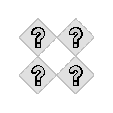
\includegraphics[scale=1]{0e0p/0e0p_double_transition_1.pdf}} \vcenteredhbox{\genarrow{1}} \vcenteredhbox{\patternimg{0.35}{0e0p_double_transition_2}}
	\caption{The $8$-state CA that we construct will work by acting on $2 \times 2$ groups of cells in such a way that applying it twice results in the same evolution (at half speed) as applying the original $2$-state CA to $3 \times 3$ groups of cells.}\label{fig:0e0p_double_transition}
\end{figure}
% TODO: Add M and N arrows in this figure?

While there are many ways that we could construct $N$, one reasonably simply approach is to ensure that if all four of its inputs comes from $\{0,7\}$ then its output is in $\{0,1,2,3,4,5,6\}$, and vice-versa. That is, we design the $8$-state CA so that patterns in even generations consist entirely of cells in the states $0$ and $7$, thus emulating the ``dead'' and ``live'' cells in a $2$-state CA, whereas in odd generations they consist entirely of cells in the state $0$ through $6$.

We first specify how $N$ should act when all of the inputs that it receives are either $0$ or $7$. Since there are only $2^4 = 16$ possible combinations of inputs in this case, we can list how $N$ acts on them explicitly:
\begin{align}\label{eq:0e0p_N_from_even}
	\begin{aligned}
		N(0,0,0,0) & = 0, \\ N(0,0,7,0) & = 4, \\ N(0,0,0,7) & = 6, \\ N(0,0,7,7) & = 1,
	\end{aligned} && \begin{aligned}
		N(7,0,0,0) & = 1, \\ N(7,0,7,0) & = 5, \\ N(7,0,0,7) & = 4, \\ N(7,0,7,7) & = 6,
	\end{aligned} && \begin{aligned}
		N(0,7,0,0) & = 2, \\ N(0,7,7,0) & = 6, \\ N(0,7,0,7) & = 3, \\ N(0,7,7,7) & = 5,
	\end{aligned} && \begin{aligned}
		N(7,7,0,0) & = 3, \\ N(7,7,7,0) & = 4, \\ N(7,7,0,7) & = 0, \\ N(7,7,7,7) & = 2.
	\end{aligned}
\end{align}
These $16$ evolution rules are displayed in Figure~\ref{fig:0e0p_rule_em}, and they do not depend at all on the rule that we are trying to emulate (i.e., these input-output combinations of $N$ are the same no matter what $M$ is).
% Emphasize that this is non-isotropic?
% TODO add an exercise to find another suitable 16 transitions. Up to permuting
% the different cell states, there are 200 different such functions sending 0 to 0.
% With 8 states we have 7 colors. Doing this with 6 or fewer colours is absolutely impossible, and with 7 colours is difficult (there are only 200 distinct solutions, or 13 up to rotation/reflection).

\begin{figure}[!htb]
	\centering
	\vcenteredhbox{\patternimg{0.25}{rule_em_0000_0}}\vcenteredhbox{\color{black}{$\xrightarrow{\text{\clock{0}{1}}}$}} \vcenteredhbox{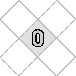
\includegraphics[scale=1]{0e0p/0e0p_rule_em_7077.pdf}} \hfill \vcenteredhbox{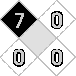
\includegraphics[scale=1]{0e0p/0e0p_rule_em_0007_0.pdf}}\vcenteredhbox{\color{black}{$\xrightarrow{\text{\clock{0}{1}}}$}} \vcenteredhbox{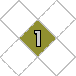
\includegraphics[scale=1]{0e0p/0e0p_rule_em_0007.pdf}} \hfill \vcenteredhbox{\patternimg{0.25}{rule_em_0070_0}}\vcenteredhbox{\color{black}{$\xrightarrow{\text{\clock{0}{1}}}$}} \vcenteredhbox{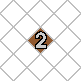
\includegraphics[scale=1]{0e0p/0e0p_rule_em_0070.pdf}} \hfill \vcenteredhbox{\patternimg{0.25}{rule_em_0077_0}}\vcenteredhbox{\color{black}{$\xrightarrow{\text{\clock{0}{1}}}$}} \vcenteredhbox{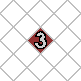
\includegraphics[scale=1]{0e0p/0e0p_rule_em_0077.pdf}} \\[1em]
	\vcenteredhbox{\patternimg{0.25}{rule_em_0700_0}}\vcenteredhbox{\color{black}{$\xrightarrow{\text{\clock{0}{1}}}$}} \vcenteredhbox{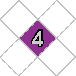
\includegraphics[scale=1]{0e0p/0e0p_rule_em_0700.pdf}} \hfill \vcenteredhbox{\patternimg{0.25}{rule_em_0707_0}}\vcenteredhbox{\color{black}{$\xrightarrow{\text{\clock{0}{1}}}$}} \vcenteredhbox{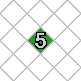
\includegraphics[scale=1]{0e0p/0e0p_rule_em_0707.pdf}} \hfill \vcenteredhbox{\patternimg{0.25}{rule_em_0770_0}}\vcenteredhbox{\color{black}{$\xrightarrow{\text{\clock{0}{1}}}$}} \vcenteredhbox{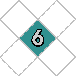
\includegraphics[scale=1]{0e0p/0e0p_rule_em_0770.pdf}} \hfill \vcenteredhbox{\patternimg{0.25}{rule_em_0777_0}}\vcenteredhbox{\color{black}{$\xrightarrow{\text{\clock{0}{1}}}$}} \vcenteredhbox{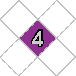
\includegraphics[scale=1]{0e0p/0e0p_rule_em_0700.pdf}} \\[1em]
	\vcenteredhbox{\patternimg{0.25}{rule_em_7000_0}}\vcenteredhbox{\color{black}{$\xrightarrow{\text{\clock{0}{1}}}$}} \vcenteredhbox{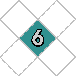
\includegraphics[scale=1]{0e0p/0e0p_rule_em_0770.pdf}} \hfill \vcenteredhbox{\patternimg{0.25}{rule_em_7007_0}}\vcenteredhbox{\color{black}{$\xrightarrow{\text{\clock{0}{1}}}$}} \vcenteredhbox{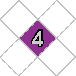
\includegraphics[scale=1]{0e0p/0e0p_rule_em_0700.pdf}} \hfill \vcenteredhbox{\patternimg{0.25}{rule_em_7070_0}}\vcenteredhbox{\color{black}{$\xrightarrow{\text{\clock{0}{1}}}$}} \vcenteredhbox{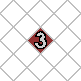
\includegraphics[scale=1]{0e0p/0e0p_rule_em_0077.pdf}} \hfill \vcenteredhbox{\patternimg{0.25}{rule_em_7077_0}}\vcenteredhbox{\color{black}{$\xrightarrow{\text{\clock{0}{1}}}$}} \vcenteredhbox{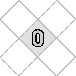
\includegraphics[scale=1]{0e0p/0e0p_rule_em_7077.pdf}} \\[1em]
	\vcenteredhbox{\patternimg{0.25}{rule_em_7700_0}}\vcenteredhbox{\color{black}{$\xrightarrow{\text{\clock{0}{1}}}$}} \vcenteredhbox{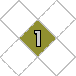
\includegraphics[scale=1]{0e0p/0e0p_rule_em_0007.pdf}} \hfill \vcenteredhbox{\patternimg{0.25}{rule_em_7707_0}}\vcenteredhbox{\color{black}{$\xrightarrow{\text{\clock{0}{1}}}$}} \vcenteredhbox{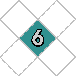
\includegraphics[scale=1]{0e0p/0e0p_rule_em_0770.pdf}} \hfill \vcenteredhbox{\patternimg{0.25}{rule_em_7770_0}}\vcenteredhbox{\color{black}{$\xrightarrow{\text{\clock{0}{1}}}$}} \vcenteredhbox{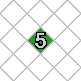
\includegraphics[scale=1]{0e0p/0e0p_rule_em_0707.pdf}} \hfill \vcenteredhbox{\patternimg{0.25}{rule_em_7777_0}}\vcenteredhbox{\color{black}{$\xrightarrow{\text{\clock{0}{1}}}$}} \vcenteredhbox{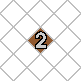
\includegraphics[scale=1]{0e0p/0e0p_rule_em_0070.pdf}}
	\caption{The rule for transitioning from even to odd generations in the $8$-state von-Neumann-neighborhood CA (rotated by 45 degrees) from Equation~\eqref{eq:0e0p_N_from_even}. The states $0$ and $7$ correspond to ``dead'' and ``alive'' in Life and are thus displayed in white and black, respectively. The states $1$, $2$, $3$, $4$, $5$, and $6$ are displayed in \bgbox{yellowback2}{yellow}, \bgbox{orangeback2}{orange}, \bgbox{redback}{red}, \bgbox{magentaback}{magenta}, \bgbox{greenpastel}{green}, and \bgbox{aquaback}{aqua}, respectively.}\label{fig:0e0p_rule_em}
\end{figure}

The reason for these seemingly-random transition rules is that they lead to the function
\[
	\begin{pmatrix}
		a_{1,1} & a_{1,2} & a_{1,3} \\
		a_{2,1} & a_{2,2} & a_{2,3} \\
		a_{3,1} & a_{3,2} & a_{3,3}
	\end{pmatrix} \mapsto \begin{pmatrix}
		N\begin{pmatrix}
		a_{1,1} & a_{1,2} \\
		a_{2,1} & a_{2,2}
		\end{pmatrix} & N\begin{pmatrix}
		a_{1,2} & a_{1,3} \\
		a_{2,2} & a_{2,3}
		\end{pmatrix} \\
		N\begin{pmatrix}
		a_{2,1} & a_{2,2} \\
		a_{3,1} & a_{3,2}
		\end{pmatrix} & N\begin{pmatrix}
		a_{2,2} & a_{2,3} \\
		a_{3,2} & a_{3,3}
		\end{pmatrix}
	\end{pmatrix}
\]
from $\{0,7\}^9$ to $\{0,1,2,3,4,5,6\}^4$ being injective (i.e., each output of the function corresponds to a \emph{unique} input). That is, given any $2 \times 2$ arrangement of states $0$, $1$, $\ldots$, $6$, we can figure out which $3 \times 3$ arrangement of $0$ and $7$ states (if any) gave rise to it. We can thus define $N$ on inputs from $\{0,1,2,3,4,5,6\}^4$ so that Equation~\eqref{eq:0e0p_N_from_M} holds.
% Mention there are other possible choices for these 16 transitions, and are found by a computer, and injectivity checked by computer

For example, [talk about emulating Life, give an example with an image, and note too many rules to list them all.]
% Mention script for computing this emulating rule: https://conwaylife.com/forums/viewtopic.php?p=38032

\begin{figure}[!htb]
	\centering
	\embedlink{0e0p_rule_em_glider}{\vcenteredhbox{\hphantom{${}\, \cdots$ \genarrow{1}}}\vcenteredhbox{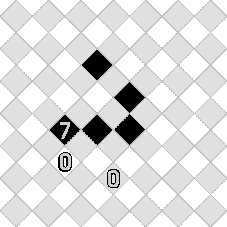
\includegraphics[scale=1]{0e0p/0e0p_glider_states0.pdf}} \vcenteredhbox{\genarrow{1}} \vcenteredhbox{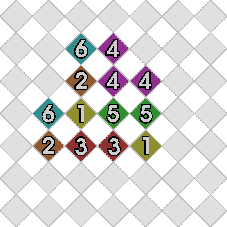
\includegraphics[scale=1]{0e0p/0e0p_glider_states.pdf}} \vcenteredhbox{\genarrow{1}} \vcenteredhbox{\patternimg{0.3}{0e0p_rule_em_glider_2}} \\[0.7em]
	\vcenteredhbox{$\cdots$ \genarrow{1}} \vcenteredhbox{\patternimg{0.3}{0e0p_rule_em_glider_3}} \vcenteredhbox{\genarrow{1}} \vcenteredhbox{\patternimg{0.3}{0e0p_rule_em_glider_4}} \vcenteredhbox{\genarrow{1}} \vcenteredhbox{\patternimg{0.3}{0e0p_rule_em_glider_5}} \\[0.7em] \vcenteredhbox{$\cdots$ \genarrow{1}} \vcenteredhbox{\patternimg{0.3}{0e0p_rule_em_glider_6}} \vcenteredhbox{\genarrow{1}} \vcenteredhbox{\patternimg{0.3}{0e0p_rule_em_glider_7}} \vcenteredhbox{\genarrow{1}} \vcenteredhbox{\patternimg{0.3}{0e0p_rule_em_glider_8}}}
	\caption{A glider from Life being emulated at half speed via an $8$-state cellular automaton using the von Neumann neighborhood (rotated by 45 degrees). Uses the same state coloring as in Figure~\ref{fig:0e0p_rule_em}.}\label{fig:0e0p_rule_em_glider}
\end{figure}

The 0E0P metacell can be programmed to emulate any of the $8^{8^4-1}$ possible zero-preserving 8-state von-Neumann-neighborhood CAs in which every cell dies every generation (not just the ones that emulate one of the $2^{2^9-1}$ zero-preserving 2-state Moore-neighborhood CAs that we are actually interested in). It takes $2^{35}$ generations for the 0E0P metacell to run one generation of the 8-state rule (emulated at a 45-degree angle), and therefore $2^{36}$ generations to emulate one generation of the corresponding 2-state Moore-neighbourhood rule (in the usual orientation).


%%%%%%%%%%%%%%%%%%%%%%%%%%%%%%%%%%%
\section{Structure of the Metacell}
%%%%%%%%%%%%%%%%%%%%%%%%%%%%%%%%%%%

\begin{figure}[htb]
	\centering
	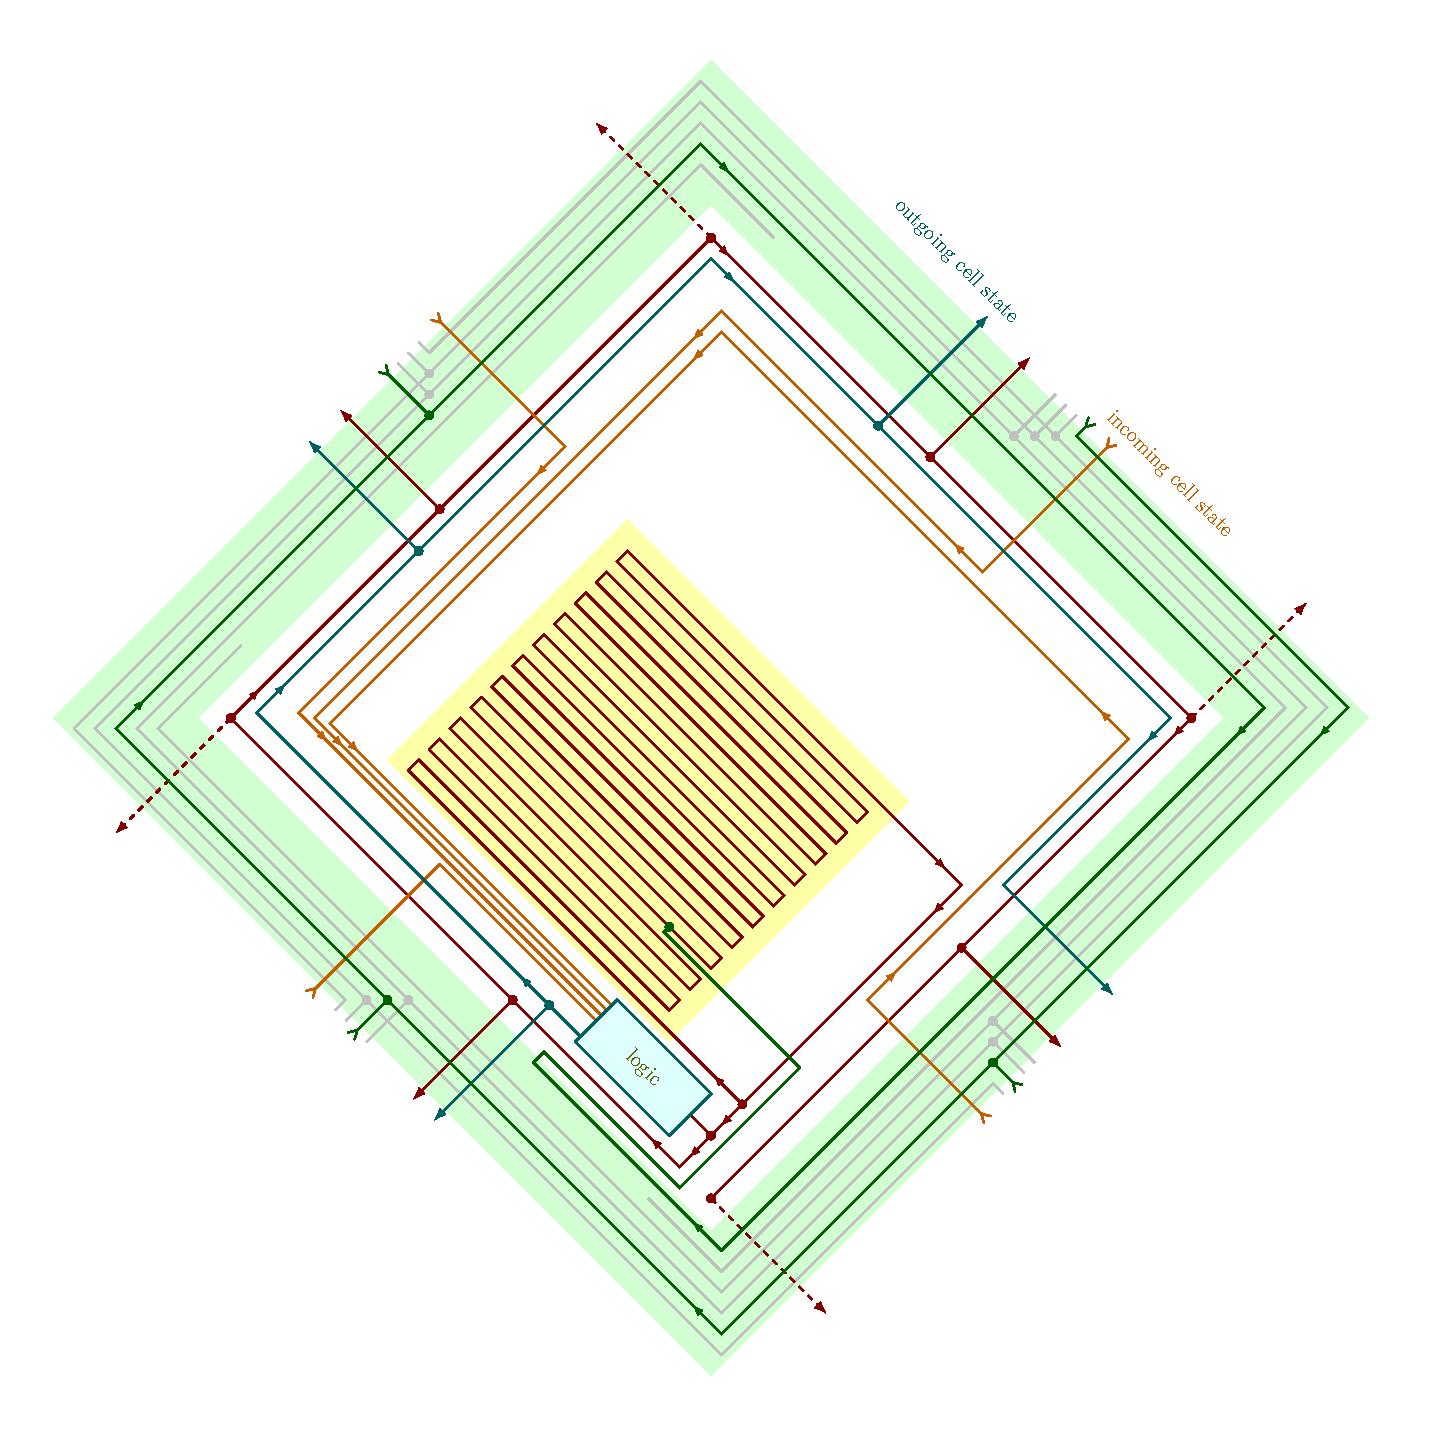
\includegraphics[width=\textwidth]{0e0p/0e0p_schematic.pdf}
	\caption{A schematic for the 0E0P metacell. The symmetrical outer
		\textbf{shell} is highlighted in pastel green, and the \textbf{nucleus}
		is highlighted in yellow. The unhighlighted region between them is the
		\textbf{kernel}.}\label{fig:0e0p_schematic}
\end{figure}

The large-scale structure of the metacell is tripartite, and each of the
three parts is constructed separately. The outer \textbf{shell} has exact
order-4 rotational symmetry, consisting of four spiral arms which propagate
gliders inwards. Only one of these arms is actually used; the other four
exist only to enforce the strict symmetry.

Inside the shell is the \textbf{kernel}, which does not have any symmetry
constraints. The south corner of the kernel contains logic circuitry for
regulating the metacell's lifecycle and computing the state of the metacell
based on the inputs from the four neighbouring cells. The kernel also contains
an output path, shown in crimson in Figure~\ref{fig:0e0p_schematic}, which
can connect to one of the four construction arms (violet, dashed) or to the
input spiral arm of one of the four neighbours. During the operation of the
metacell, the glider stream is redirected between the different possible
outputs by deleting Snarks.

The largest region of the metacell is the \textbf{nucleus}, a huge
boustrophedonic glider loop with a period of exactly $2^{29}$. The nucleus
is populated by over three million gliders, which together encode all of
the construction recipes along with the lookup table for the metacell's rule.

%%%%%%%%%%%%%%%%%%%%%
\section{Memory Tape}
%%%%%%%%%%%%%%%%%%%%%

Stuff.

%%%%%%%%%%%%%%%%%%%%%%%%%
\section{Logic Circuitry}
%%%%%%%%%%%%%%%%%%%%%%%%%

Stuff.

%%%%%%%%%%%%%%%%%%%%%%
\section{Construction}
%%%%%%%%%%%%%%%%%%%%%%

Stuff.


%%%%%%%%%%%%%%%%%%%%%%%%%%%%%%%%
\section{Notes and Historical Remarks}\label{sec:0e0p_history}\index{metacell}
%%%%%%%%%%%%%%%%%%%%%%%%%%%%%%%%

Many metacells---patterns of size larger than $1 \times 1$ that emulate the behavior of a single cell---were constructed prior to 0E0P. The first one was the \textbf{p5760~metacell}, which was constructed by David Bell in January 1996. This metacell is much smaller and faster than 0E0P, with a period of just $5760$~generations and a bounding box size of just $500 \times 500$ (see Figure~\ref{fig:p5760_metacell}). However, there are numerous trade-offs that make this metacell less useful:\smallskip

\begin{figure}[!htb]
	\centering
	\begin{tikzpicture}
	\node[inner sep=0pt,anchor=south west] at (0,0) {\embedlink{p5760_metacell}{\patternimg{0.15}{p5760_metacell}}};
	
	\draw[white,line width=2.5pt,opacity=0.6](2.63,8.15) circle (0.2);
	\draw[redback2,line width=1pt](2.63,8.15) circle (0.2);
	\end{tikzpicture}
	\caption{The \emph{p$5760$~metacell}. Whether the cell is considered ``alive'' or ``dead'' is determined by the presence or absence of a glider at the location circled in \bgbox{redback}{red}. That glider, if present, is duplicated $8$ times and sent to its neighbors along the $8$ output paths highlighted in \bgbox{aquaback}{aqua}, signaling to them that it is alive. Similarly, neighboring alive cells send their signals to this one along the input paths highlighted in \bgbox{magentaback}{magenta}.}\label{fig:p5760_metacell}
\end{figure}

\begin{itemize}
	\item[1)] It is hard-wired to emulate Life, and cannot easily be modified to emulate most of the $2^{512}$ different non-isotropic Life-like cellular automata.\smallskip
	
	\item[2)] It is not easy to tell at a glance which ``cells'' are alive and which are dead---it is determined by the presence or absence of a single extra glider in the cell---and thus is not interesting to look at from a far-out zoom level.\smallskip
	
	\item[3)] ``Dead'' cells must be placed on the Life plane, which means that, for example, spaceships cannot be emulated by this metacell unless the pattern is infinitely large.\smallskip
\end{itemize}

The first two of these problems were solved by the \emph{OTCA metapixel},\index{OTCA metapixel} which was constructed by Brice Due from late 2005 to mid-2006. While this metacell is a bit larger and slower than the first metacell (it is $2048 \times 2048$ and has period $35{\thousep}328$), it can be used to emulate any of the $2^{18}$ different outer-totalistic Life-like cellular automata. Indeed, built into its circuitry is an easily-adjustable array of eaters that determine how many live neighboring OTCA metapixels should lead to the birth or survival of the current metapixel (see Figure~\ref{fig:otca_metapixel}). 
% Introduce Life-like CA, since no introduction earlier
% mention out of the blue/honey bit/demultiplexer?

% FIGURE HERE, SHOWING PIXEL AND RULE ENCODINGS

The OTCA metapixel also has the remarkable feature that its alive and dead states look, from a distance, like alive and dead cells. This feature is achieved by the ``alive'' version of the cell releasing $43$ pairs of perpendicular lightweight spaceship streams that mutually annihilate each other, thus partially filling in the otherwise empty center of the metacell. For example, arranging a $1 \times 3$ row of ``alive'' metapixels (and a suitably large ``dead'' array of metapixels around its edges) results in a pattern that looks and evolves like a blinker, but $2{\thousep}048$ times as long and wide and $35{\thousep}328$ times as slow (see Figure~\ref{fig:metablinker}).

\begin{figure}[!htb]
	\centering
	\embedlink{metablinker}{\vcenteredhbox{\patternimg{0.104}{metablinker_0}} \vcenteredhbox{\color{black}{$\xrightarrow{\text{\clock{5}{46} 35328}}$}} \vcenteredhbox{\patternimg{0.104}{metablinker_35328}}}
	\caption{A \emph{metablinker}: an arrangement of OTCA metapixels that emulates a blinker, but with period $2 \times 35{\thousep}328$.}\label{fig:metablinker}\index{metablinker}
\end{figure}

The next notable metacell to be constructed was the \emph{p1 megacell},\index{p1 megacell} by Adam P.~Goucher in 2008. This metacell was, again, larger and slower than the metacells that came before it, with a bounding box of $2^{15} \times 2^{15}$ and a period of $2^{24}$. The new features this time that warranted the extra size and delay were twofold:\smallskip

\begin{itemize}
	\item This metacell was built entirely out of stable (p$1$) components like Herschel tracks, with the exception of a single period~$2^{24}$ gun used to regulate its timing.\footnote{This gun could be swapped out for a gun of another period, but periods that are multiples of $2$ help the pattern run quicker under the HashLife algorithm in Life simulation software like Golly.}\index{HashLife}\smallskip
	
	\item All $2^{512}$ non-outer-totalistic Life-like cellular automata can be emulated by this metacell, versus the $2^{18}$ outer-totalistic Life-like cellular automata that can be emulated by the OTCA metapixel.\smallskip% Maybe not-necessarily-outer-totalistic, instead of non-outer-totalistic?
\end{itemize}

% Figure of p1 megacell? Have had a lot of big figures bunched up closely here, so maybe not.

Finally, Adam P.~Goucher spent 2014--2018 constructing the 0E0P metapixel, which solved problem~(3) described earlier---it does not require a background grid of ``dead'' cells to be placed on the Life plane.

%https://www.conwaylife.com/forums/viewtopic.php?f=15&t=4117#p82954
%https://cp4space.hatsya.com/2018/11/12/fully-self-directed-replication/
%https://www.conwaylife.com/forums/viewtopic.php?f=2&t=3835
%https://www.conwaylife.com/forums/viewtopic.php?t=3968

% EXERCISE: Give reactions in HighLife-replicator-ship.rle from Golly and ask reader to make ship out of it
% EXERCISE: Logarithmic replicator from B36/S245, found by Mark Niemiec in July 1994. Do... something with it. Pop in generation 300*4^n - 127 is 64 for all n >= 0.


%%%%%%%%%%%%%%%%%%%%%%%%%%%%%%%%%
\section*{Exercises \hfill \normalfont\textsf{\small solutions to starred exercises on \hyperlink{solutions_0e0p}{page \pageref{solutions_0e0p}}}}
\label{sec:solutions_0e0p}
\addcontentsline{toc}{section}{Exercises}
\vspace*{-0.4cm}\hrulefill\vspace*{-0.3cm}\footnotesize\begin{multicols}{2}\vspace*{-0.4cm}\raggedcolumns\interlinepenalty=10000
	\setlength{\parskip}{0pt}
	%%%%%%%%%%%%%%%%%%%%%%%%%%%%%%%%%
	
	
	\begin{problem}\label{exer:0e0p_hamming_weight} \probdiff{1}
		Construct a formula for the population of the replicator from Figure~\ref{fig:highlife_replicator} in generation $12n$, where $n \geq 0$ is an integer. You may use the \emph{Hamming weight}\index{Hamming weight} of $n$, denoted by $H(n)$, which counts the number of ``1'' bits in the binary representation of $n$.
	\end{problem}


	\mfilbreak
	
	
	\begin{problem}\label{exer:replicator_rule_really_replicates}
		Recall the replicator rule B1357/S1357 that was illustrated in Figure~\ref{fig:replicator_smile}.
		
		\begin{enumerate}[label=\bf\color{ocre}(\alph*)]
			\item \probdiff{2} If the longest side of a pattern's bounding box is $n$ cells long, how many generations would it take to copy itself for the first time in this rule?
			% Solution: 2^(ceil(log_2(n))) generations
			
			\item \probdiff{5} Prove that every pattern in this rule really does replicate, as we claimed.
			
			\noindent [Hint: First, prove (via induction, perhaps) that a single cell replicates. Then show that evolving a multi-cell pattern in this rule is equivalent to evolving each cell individually and XOR-ing the results together.].
		\end{enumerate}
	\end{problem}
	
	
	%% EXERCISE END COMMANDS
\end{multicols}
\normalsize\vspace*{0.01cm}
%% DONE EXERCISE END COMMANDS
